% uOttawa  Thesis Template for LaTeX 
% Edited by Manuel Ferrer based on Wail Gueaieb's edit on the uWaterloo's Template
% Last Updated October 2026

% This is mainly a repackaging of their thesis template. 



% Please read the "00readme.txt" file first.
%
% DON'T FORGET TO ADD YOUR OWN NAME AND TITLE in the "hyperref" package
% configuration below. THIS INFORMATION GETS EMBEDDED IN THE PDF FINAL PDF DOCUMENT.
% You can view the information if you view Properties of the PDF document.

% The template is based on the standard "book" document class which provides 
% all necessary sectioning structures and allows multi-part theses.

% DISCLAIMER
% To the best of our knowledge, this template satisfies the current 
% uOttawa thesis requirements.
% However, it is your responsibility to assure that you have met all 
% requirements of the university and your particular department.

% -----------------------------------------------------------------------

% By default, output is produced that is geared toward generating a PDF 
% version optimized for viewing on an electronic display, including 
% hyperlinks within the PDF.
 
% E.g. to process a thesis called "mythesis.tex" based on this template, run:

% pdflatex mythesis	-- first pass of the pdflatex processor
% bibtex mythesis	-- generates bibliography from .bib data file(s)
% makeindex         -- should be run only if an index is used 
% pdflatex mythesis	-- fixes numbering in cross-references, bibliographic references, glossaries, index, etc.
% pdflatex mythesis	-- fixes numbering in cross-references, bibliographic references, glossaries, index, etc.

% If you use the recommended LaTeX editor, Texmaker, you would open the mythesis.tex
% file, then click the PDFLaTeX button. Then run BibTeX (under the Tools menu).
% Then click the PDFLaTeX button two more times. If you have an index as well,
% you'll need to run MakeIndex from the Tools menu as well, before running pdflatex
% the last two times.

% N.B. The "pdftex" program allows graphics in the following formats to be
% included with the "\includegraphics" command: PNG, PDF, JPEG, TIFF
% Tip 1: Generate your figures and photos in the size you want them to appear
% in your thesis, rather than scaling them with \includegraphics options.
% Tip 2: Any drawings you do should be in scalable vector graphic formats:
% SVG, PNG, WMF, EPS and then converted to PNG or PDF, so they are scalable in
% the final PDF as well.
% Tip 3: Photographs should be cropped and compressed so as not to be too large.

% To create a PDF output that is optimized for double-sided printing: 
%
% 1) comment-out the \documentclass statement in the preamble below, and
% un-comment the second \documentclass line.
%
% 2) change the value assigned below to the boolean variable
% "PrintVersion" from "false" to "true".

% --------------------- Start of Document Preamble -----------------------

% Specify the document class, default style attributes, and page dimensions
% For hyperlinked PDF, suitable for viewing on a computer, use this:
\documentclass[letterpaper,12pt,titlepage,oneside,final]{book}
 
% For PDF, suitable for double-sided printing, change the PrintVersion variable below
% to "true" and use this \documentclass line instead of the one above:
%\documentclass[letterpaper,12pt,titlepage,openright,twoside,final]{book}

% Some LaTeX commands I define for my own nomenclature.
% If you have to, it's better to change nomenclature once here than in a 
% million places throughout your thesis!
\newcommand{\package}[1]{\textbf{#1}} % package names in bold text
\newcommand{\cmmd}[1]{\textbackslash\texttt{#1}} % command name in tt font 
\newcommand{\href}[1]{#1} % does nothing, but defines the command so the
    % print-optimized version will ignore \href tags (redefined by hyperref pkg).
%\newcommand{\texorpdfstring}[2]{#1} % does nothing, but defines the command
% Anything defined here may be redefined by packages added below...

% This package allows if-then-else control structures.
\usepackage{ifthen}
\newboolean{PrintVersion}
\setboolean{PrintVersion}{false} 
% CHANGE THIS VALUE TO "true" as necessary, to improve printed results for hard copies
% by overriding some options of the hyperref package below.

% \usepackage{nomencl} % For a nomenclature (optional; available from ctan.org)


% Citation packages
\usepackage{cite}  % For better handling of numeric citations

% Math packages
\usepackage{amsmath,amssymb,amstext,amsfonts} % Lots of math symbols and environments
\usepackage{mathtools}
\usepackage{siunitx}  % To type units
%\sisetup{unitsep=tightcdot}
\usepackage{physics}  % Convenient for many mathematical notations
\usepackage{dsfont}
%
\usepackage{amsthm}  % to create theorem-like environments
\newtheorem{lemma}{Lemma}[chapter]
\newtheorem{theorem}{Theorem}[chapter]
\newtheorem{corollary}{Corollary}[chapter]
\newtheorem{definition}{Definition}[chapter]



% Graphic packages
\usepackage[pdftex]{graphicx} % For including graphics N.B. pdftex graphics driver
% To arrange subfigures within the same figure, it is
% recommended to use the package subcaption instead of
% packages subfig or subfigure, for example.
\usepackage{caption}
\usepackage{subcaption}
\captionsetup[sub]{subrefformat=parens, skip=2pt}

% Includes pdfs 
\usepackage{pdfpages}

% Table packages
\usepackage{booktabs}  % Nice looking tables


% Algorithm packages
% It is recommended to use algorithmx, as done below, instead of
% using package algorithm2e, for instance.
\usepackage{algorithm,algpseudocode,float}
\renewcommand{\algorithmicrequire}{\textbf{Input:}}
\renewcommand{\algorithmicensure}{\textbf{Output:}}
\algnewcommand{\algorithmicand}{\textbf{ and }}
\algnewcommand{\algorithmicor}{\textbf{ or }}
\algnewcommand{\algAnd}{\algorithmicand}
\algnewcommand{\algOr}{\algorithmicor}

\makeatletter
\@addtoreset{algorithm}{chapter}% algorithm counter resets every chapter
\makeatother
\renewcommand{\thealgorithm}{\arabic{chapter}.\arabic{algorithm}}


%=== ADD MORE PACKAGES AS NEEDED. TYPICALLY, hyperref (INCLUDED BELOW)
%=== IS THE LAST PACKAGE TO BE LOADED 





%====================================================


% Hyperlinks make it very easy to navigate an electronic document.
% In addition, this is where you should specify the thesis title
% and author as they appear in the properties of the PDF document.
% Use the "hyperref" package 
% N.B. HYPERREF MUST BE THE LAST PACKAGE LOADED; ADD ADDITIONAL PKGS ABOVE
\usepackage[pdftex,pagebackref=false]{hyperref} % with basic options
		% N.B. pagebackref=true provides links back from the References to the body text. This can cause trouble for printing.
\hypersetup{
    plainpages=false,       % needed if Roman numbers in frontpages
    unicode=false,          % non-Latin characters in Acrobat’s bookmarks
    pdftoolbar=true,        % show Acrobat’s toolbar?
    pdfmenubar=true,        % show Acrobat’s menu?
    pdffitwindow=false,     % window fit to page when opened
    pdfstartview={FitH},    % fits the width of the page to the window
    pdftitle={QuantumThesisuOttawa},    % title: CHANGE THIS TEXT!
%    pdfauthor={Author},    % author: CHANGE THIS TEXT! and uncomment this line
%    pdfsubject={Subject},  % subject: CHANGE THIS TEXT! and uncomment this line
%    pdfkeywords={keyword1} {key2} {key3}, % list of keywords, and uncomment this line if desired
    pdfnewwindow=true,      % links in new window
    colorlinks=true,        % false: boxed links; true: colored links
    linkcolor=blue,         % color of internal links
    citecolor=green,        % color of links to bibliography
    filecolor=magenta,      % color of file links
    urlcolor=titlecolor2        % color of external links
}
\ifthenelse{\boolean{PrintVersion}}{   % for improved print quality, change some hyperref options
\hypersetup{	% override some previously defined hyperref options
%    colorlinks,%
    citecolor=black,%
    filecolor=black,%
    linkcolor=black,%
    urlcolor=black}
}{} % end of ifthenelse (no else)

\usepackage[noabbrev]{cleveref}  % automatically sort references

\usepackage[automake,toc,abbreviations]{glossaries-extra} % Exception to the rule of hyperref being the last add-on package
% If glossaries-extra is not in your LaTeX distribution, get it from CTAN (http://ctan.org/pkg/glossaries-extra), 
% although it's supposed to be in both the TeX Live and MikTeX distributions. There are also documentation and 
% installation instructions there.

% Setting up margins and other spaces 
% Setting up the page margins...
% uWaterloo thesis requirements specify a minimum of 1 inch (72pt) margin at the
% top, bottom, and outside page edges and a 1.125 in. (81pt) gutter
% margin (on binding side). While this is not an issue for electronic
% viewing, a PDF may be printed, and so we have the same page layout for
% both printed and electronic versions, we leave the gutter margin in.
% Set margins to minimum permitted by uWaterloo thesis regulations:
\setlength{\marginparwidth}{0pt} % width of margin notes
% N.B. If margin notes are used, you must adjust \textwidth, \marginparwidth
% and \marginparsep so that the space left between the margin notes and page
% edge is less than 15 mm (0.6 in.)
\setlength{\marginparsep}{0pt} % width of space between body text and margin notes
\setlength{\evensidemargin}{0.125in} % Adds 1/8 in. to binding side of all 
% even-numbered pages when the "twoside" printing option is selected
\setlength{\oddsidemargin}{0.125in} % Adds 1/8 in. to the left of all pages
% when "oneside" printing is selected, and to the left of all odd-numbered
% pages when "twoside" printing is selected
\setlength{\textwidth}{6.375in} % assuming US letter paper (8.5 in. x 11 in.) and 
% side margins as above
\raggedbottom

% The following statement specifies the amount of space between
% paragraphs. Other reasonable specifications are \bigskipamount and \smallskipamount.
\setlength{\parskip}{\medskipamount}

% The following statement controls the line spacing.  The default
% spacing corresponds to good typographic conventions and only slight
% changes (e.g., perhaps "1.2"), if any, should be made.
\renewcommand{\baselinestretch}{1} % this is the default line space setting


 


% By default, each chapter will start on a recto (right-hand side)
% page.  We also force each section of the front pages to start on 
% a recto page by inserting \cleardoublepage commands.
% In many cases, this will require that the verso page be
% blank and, while it should be counted, a page number should not be
% printed.  The following statements ensure a page number is not
% printed on an otherwise blank verso page.
\let\origdoublepage\cleardoublepage
\newcommand{\clearemptydoublepage}{%
  \clearpage{\pagestyle{empty}\origdoublepage}}
\let\cleardoublepage\clearemptydoublepage

% Define Glossary terms (This is properly done here, in the preamble. Could be \input{} from a file...)
%% Main glossary entries -- definitions of relevant terminology
\newglossaryentry{computer}
{
name=computer,
description={A programmable machine that receives input data,
               stores and manipulates the data, and provides
               formatted output}
}

% Nomenclature glossary entries -- New definitions, or unusual terminology
\newglossary*{nomenclature}{Nomenclature}
\newglossaryentry{dingledorf}
{
type=nomenclature,
name=dingledorf,
description={A person of supposed average intelligence who makes incredibly brainless misjudgments}
}

% List of Abbreviations (abbreviations type is built in to the glossaries-extra package)
\newabbreviation{aaaaz}{AAAAZ}{American Association of Amature Astronomers and Zoologists}

% List of Symbols
\newglossary*{symbols}{List of Symbols}
\newglossaryentry{rvec}
{
name={$\mathbf{v}$},
sort={label},
type=symbols,
description={Random vector: a location in n-dimensional Cartesian space, where each dimensional component is determined by a random process}
}
  
%\makeglossaries

%\usepackage{empheq}


%% Including the Bolded Mathcal txt
\DeclareMathAlphabet\mathbfcal{OMS}{cmsy}{b}{n}

\usepackage{selinput}
\SelectInputMappings{%
  aacuttee={á},
  ntilde={ñ},
  Euro={€}
}



%%%%%
\usepackage{babel}
\usepackage{beramono}
\usepackage[T1]{fontenc}
%\usepackage[dvisvgm, usenames, dvipsnames]{color}
%\usepackage[latin9]{inputenc}
%\usepackage{}{color}

\definecolor{titlecolor}{rgb}{1,0.44,0.44}
\definecolor{titlecolor2}{rgb}{0.06,0.47,0.69}

\definecolor{identifiercolor}{rgb}{.4,.6,.56}
\definecolor{stringcolor}{gray}{0.5}
\definecolor{inactivecolor}{rgb}{0.15,0.15,0.5}
\usepackage{listings}
\lstset{basicstyle={\footnotesize\def\fvm@Scale{.85}\fontfamily{fvm}\selectfont},
  breaklines=true,
  escapeinside={\%*}{*)},
  keywordstyle={\bfseries\color{inactivecolor}},
  stringstyle={\bfseries\color{stringcolor}},
  identifierstyle={\bfseries\color{identifiercolor}},
  language=Mathematica,
  otherkeywords={DiscretizeRegion},
  showstringspaces=false}
\renewcommand{\lstlistingname}{Listing}

%----------------------------------------------------------------------
% Including Publications easily
%----------------------------------------------------------------------
\newcommand{\Publication}[2]{
\newpage
 \par\refstepcounter{section}% Increase section counter
  \sectionmark{#1}% Add section mark (header)
  \addcontentsline{toc}{section}{\protect\numberline{\thesection}#1}% Add section to ToC
  \includepdf[pages={-},pagecommand={}]{#2} 
  % Add more content here, if needed.
}




%======================================================================
%   L O G I C A L    D O C U M E N T -- the content of your thesis
%======================================================================
\begin{document}
% For a large document, it is a good idea to divide your thesis
% into several files, each one containing one chapter.
% To illustrate this idea, the "front pages" (i.e., title page,
% declaration, borrowers' page, abstract, acknowledgements,
% dedication, table of contents, list of tables, list of figures,
% nomenclature) are contained within the file "uw-ethesis-frontpgs.tex" which is
% included into the document by the following statement.
%----------------------------------------------------------------------
% FRONT MATERIAL
%----------------------------------------------------------------------



\newcommand{\thesisauthor}{Your Name Here}
\newcommand{\thesistitlecoverpage}{%
  Awesome Title
}
\newcommand{\thesisdegree}{Doctor of Philosophy} % possible values are:
                            % Master of Applied Science / Master 
\newcommand{\nameofprogram}{Physics}
\newcommand{\graduationyear}{20XX}

% T I T L E   P A G E
% -------------------
% Last updated June 14, 2017, by Stephen Carr, IST-Client Services
% The title page is counted as page `i' but we need to suppress the
% page number. Also, we don't want any headers or footers.
\pagestyle{empty}
\pagenumbering{roman}

% F R O N T   P A G E
% -------------------------------

% The contents of the title page are specified in the "titlepage"
% environment.
\begin{titlepage}
        \begin{center}
        \vspace*{1.0cm}

        \Huge
        {\bf \thesistitlecoverpage}

        \vspace*{1.0cm}

        \normalsize
        by \\

        \vspace*{1.0cm}

        \Large
        \thesisauthor \\

        \vspace*{3.0cm}

        \normalsize
        A thesis \\
        submitted to the University of Ottawa \\ 
        in partial fulfillment of the \\
        thesis requirement for the degree of \\
        \thesisdegree \\
        in \\
        \nameofprogram \\

        \vspace*{3.0cm}


        \copyright\ {\thesisauthor}, Ottawa, Canada, \graduationyear \\
        \end{center}
\end{titlepage}



% The rest of the front pages should contain no headers and be numbered using Roman numerals starting with `ii'
\pagestyle{plain}
\setcounter{page}{2}

\cleardoublepage % Ends the current page and causes all figures and tables that have so far appeared in the input to be printed.
% In a two-sided printing style, it also makes the next page a right-hand (odd-numbered) page, producing a blank page if necessary.

% A B S T R A C T
% ---------------
\addcontentsline{toc}{chapter}{\textbf{Abstract}}
\begin{Huge}
\noindent \textbf{Abstract\\}\end{Huge}
\vspace{0.7cm}

This is a placeholder abstract. Replace this text with a concise summary of your thesis, including the motivation for the work, the methods used, the main results, and the most important conclusions.

In this thesis, we investigate an extremely important scientific problem using a collection of very sophisticated methods. Several experiments are performed, many equations are solved, and a non-negligible amount of coffee is consumed. The results show that something interesting happens under certain conditions, in reasonable agreement with expectations. These findings provide new insight into the problem and suggest several exciting directions for future work.

Seriously, replace this abstract before submitting your thesis.


\cleardoublepage

% A C K N O W L E D G E M E N T S
% -------------------------------
\addcontentsline{toc}{chapter}{\textbf{Acknowledgments}}
\begin{Huge}
\noindent \textbf{Acknowledgments \\}\end{Huge}
\vspace{0.7cm}

This is a placeholder acknowledgements section. Replace this text with your own acknowledgements before submitting your thesis.

You may wish to thank your supervisor, committee members, collaborators, laboratory colleagues, funding agencies, friends, family, and anyone else who supported you during your degree.

For example, you could write something thoughtful about your supervisor's guidance, your colleagues' helpful discussions, and your family's support. You could also acknowledge the indispensable contributions of coffee, late-night snacks, and the one piece of laboratory equipment that only works when nobody is watching.

Seriously, though—replace this text. If you are reading this in your submitted thesis, it is already too late.





\cleardoublepage


% D E D I C A T I O N
% -------------------

\noindent \textit{Research is what I’m doing when I don’t know what I’m doing.} \\ Placeholder Researcher

\cleardoublepage


% L I S T   O F   T A B L E S
% ---------------------------
\addcontentsline{toc}{chapter}{List of Publications}
\renewcommand{\listtablename}{List of Publications}
\listoftables
\begin{enumerate}
    \item A. N. Author, \textbf{S. T. U. Dent}, and P. H. D. Advisor, 
    ``A very important investigation of an extremely interesting physical phenomenon.'' 
    \textit{Journal of Placeholder Physics} \textbf{42}, 100--110 (2023).

    \item \textbf{S. T. U. Dent}, A. N. Author, and P. H. D. Advisor, 
    ``Experimental observation of something that was theoretically expected to happen.'' 
    \textit{International Journal of Dummy Research} \textbf{17}, 123456 (2024).

    \item \textbf{S. T. U. Dent}, C. O. Author, A. N. Author, and P. H. D. Advisor, 
    ``Further studies on the propagation of light, knowledge, and uncertainty.'' 
    \textit{Proceedings of Imaginary Optics} \textbf{99}, 200--208 (2025).
\end{enumerate}
\phantomsection		% allows hyperref to link to the correct page

\cleardoublepage

% D E C L A R A T I O N   P A G E
% -------------------------------
\addcontentsline{toc}{chapter}{Statement of originality and collaborative contributions}
\begin{Huge}

\noindent \textbf{Statement of originality and \\[1ex]collaborative contributions} \end{Huge}
\vspace{0.7cm}

To the best of the author's knowledge, the work described in this thesis constitutes original research in the field of physics. The collaborative contributions of the authors to the work presented in each chapter are described below.

Supervisor 1 and Supervisor 2 conceived the idea for the work presented in Chapter~\ref{Ch:LightAndFocusing}, concerning the study of good photons. Author 1 performed the numerical simulations and analyzed the resulting data. Author 1 and Supervisor 2 prepared the manuscript with contributions from all authors. All authors discussed the results and contributed to the final version of the manuscript.

Supervisor 1 and Author 2 conceived the idea for the work presented in Chapter~\ref{Ch:wave&Weak}, concerning stars on waveguides and weak measurements. Author 1 and Author 2 designed the optical fields. Author 1 performed the numerical simulations, while Author 1 and Author 2 analyzed the resulting data. Author 1, Author 2, and Supervisor 1 prepared the manuscript with contributions from all authors. All authors discussed the results and contributed to the final version of the manuscript.


\cleardoublepage

% L I S T   O F   F I G U R E S
% -----------------------------
\addcontentsline{toc}{chapter}{List of Figures}
\listoffigures
\cleardoublepage
\phantomsection		% allows hyperref to link to the correct page


% T A B L E   O F   C O N T E N T S
% ---------------------------------
  \tableofcontents
\cleardoublepage
\phantomsection    % allows hyperref to link to the correct page



% GLOSSARIES (Lists of definitions, abbreviations, symbols, etc. provided by the glossaries-extra package)
% -----------------------------
%\printglossaries
\cleardoublepage
\phantomsection		% allows hyperref to link to the correct page

% Change page numbering back to Arabic numerals
\pagenumbering{arabic}

 

%----------------------------------------------------------------------
% MAIN BODY
%----------------------------------------------------------------------
% Because this is a short document, and to reduce the number of files
% needed for this template, the chapters are not separate
% documents as suggested above, but you get the idea. If they were
% separate documents, they would each start with the \chapter command, i.e, 
% do not contain \documentclass or \begin{document} and \end{document} commands.
%======================================================================
\input{src/C1:Introduction} 
\input{src/C2:Chapter2} 
\input{src/C3:Chapter3}
%======================================================================
\chapter{Conclusions}
%======================================================================

In this thesis, several aspects of light and optical systems were investigated using theoretical, numerical, and experimental methods. The results presented throughout the different chapters illustrate how fundamental concepts in optics can be applied to study a variety of physical systems.

The work discussed here provides a general example of how a thesis conclusion may summarize the main results, highlight their significance, and identify possible directions for future research.

This is placeholder text. Replace this section with a concise summary of the main contributions of your thesis, the conclusions supported by your results, and any relevant future perspectives.


% The \appendix statement indicates the beginning of the appendices.
\appendix
% Add a title page before the appendices and a line in the Table of Contents
\chapter*{APPENDICES}
\addcontentsline{toc}{chapter}{APPENDICES}
%======================================================================
% An appendix
\chapter[Numerical calculations]{Numerical calculation of something}
\label{AppendixA}
% Tip 4: Example of how to get a shorter chapter title for the Table of Contents 
%======================================================================
In this section, we provide the ... notebooks used for the calculation of... 

\section{Code 1: Mathematica version}
\subsection{Main code}



\noindent\textcolor{titlecolor2}{\textbf{\textsf{Definition }}}
\begin{lstlisting}[extendedchars=true,language=Mathematica]
(* Plot something easy *) 
intensity[x_] := Exp[-x^2]

Plot[intensity[x], {x, -3, 3}]

\end{lstlisting}


\section{Python}
\subsection{Main code }
\begin{lstlisting}[language=Python]
import numpy as np
import matplotlib.pyplot as plt

def intensity(x):
    return np.exp(-x**2)

x = np.linspace(-3, 3, 300)
plt.plot(x, intensity(x))
plt.show()
\end{lstlisting}
%======================================================================
\chapter{Supplementary Materials: SM1}
\label{AppendixB}
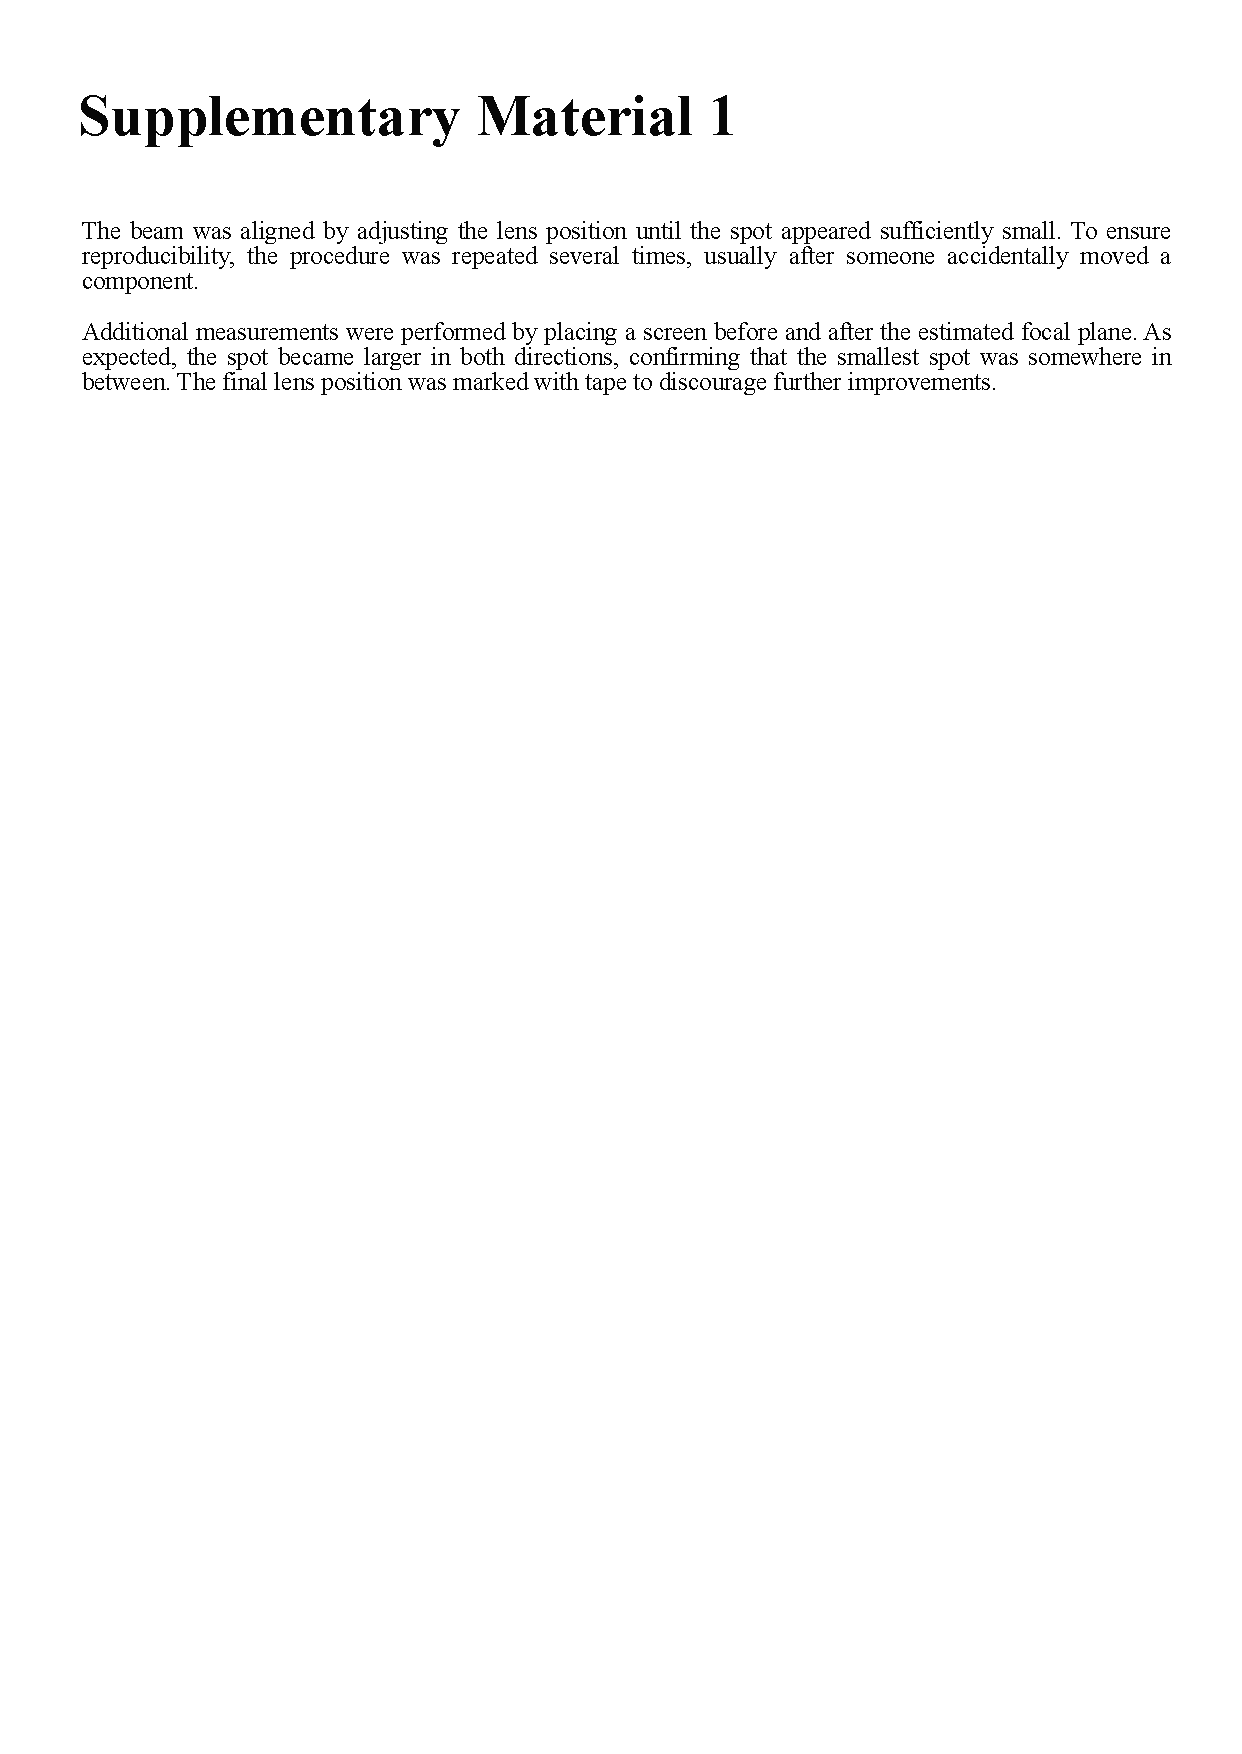
\includepdf[pages=-,pagecommand={}]{PDF/SM1.pdf} 


%======================================================================
\chapter{Supplementary Materials: SM2}
\label{AppendixC}
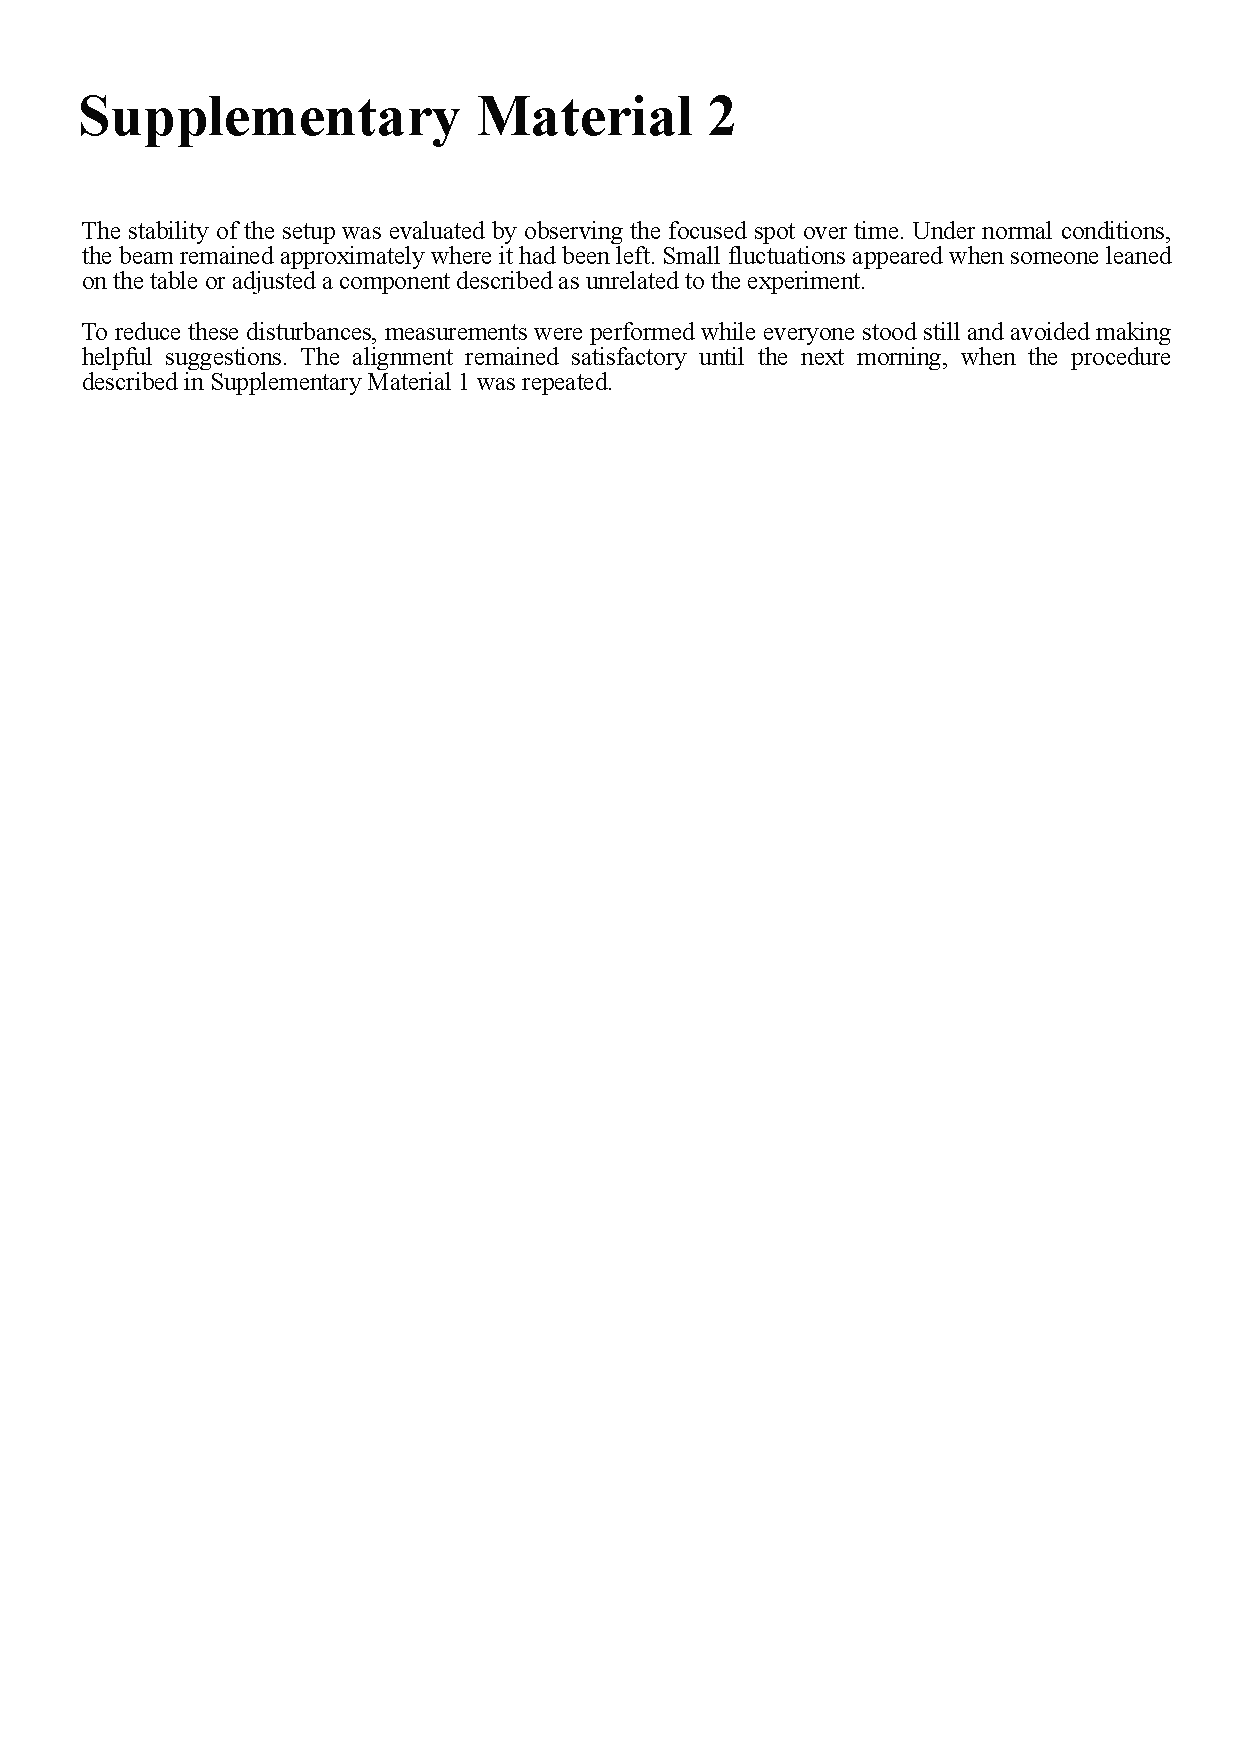
\includepdf[pages=-,pagecommand={}]{PDF/SM2.pdf} 
 
%----------------------------------------------------------------------
% END MATERIAL
%----------------------------------------------------------------------

% B I B L I O G R A P H Y
% -----------------------

% The following statement selects the style to use for references.  It controls the sort order of the entries in the bibliography and also the formatting for the in-text labels.
\bibliographystyle{unsrt}
% This specifies the location of the file containing the bibliographic information.  
% It assumes you're using BibTeX (if not, why not?).
\cleardoublepage % This is needed if the book class is used, to place the anchor in the correct page,
                 % because the bibliography will start on its own page.
                 % Use \clearpage instead if the document class uses the "oneside" argument
\phantomsection  % With hyperref package, enables hyperlinking from the table of contents to bibliography             
% The following statement causes the title "References" to be used for the bibliography section:
\renewcommand*{\bibname}{References}

% Add the References to the Table of Contents
\addcontentsline{toc}{chapter}{\textbf{References}}

\bibliography{bibliography/uo-ethesis}
% Tip 5: You can create multiple .bib files to organize your references. 
% Just list them all in the \bibliogaphy command, separated by commas (no spaces).

% The following statement causes the specified references to be added to the bibliography% even if they were not 
% cited in the text. The asterisk is a wildcard that causes all entries in the bibliographic database to be included (optional).
% \nocite{*}



\end{document}


%%% Local Variables:
%%% mode: latex
%%% TeX-master: t
%%% End:
